\PassOptionsToPackage{unicode=true}{hyperref} % options for packages loaded elsewhere
\PassOptionsToPackage{hyphens}{url}
%
\documentclass[]{article}
\usepackage{lmodern}
\usepackage{amssymb,amsmath}
\usepackage{ifxetex,ifluatex}
\usepackage{fixltx2e} % provides \textsubscript
\ifnum 0\ifxetex 1\fi\ifluatex 1\fi=0 % if pdftex
  \usepackage[T1]{fontenc}
  \usepackage[utf8]{inputenc}
  \usepackage{textcomp} % provides euro and other symbols
\else % if luatex or xelatex
  \usepackage{unicode-math}
  \defaultfontfeatures{Ligatures=TeX,Scale=MatchLowercase}
\fi
% use upquote if available, for straight quotes in verbatim environments
\IfFileExists{upquote.sty}{\usepackage{upquote}}{}
% use microtype if available
\IfFileExists{microtype.sty}{%
\usepackage[]{microtype}
\UseMicrotypeSet[protrusion]{basicmath} % disable protrusion for tt fonts
}{}
\IfFileExists{parskip.sty}{%
\usepackage{parskip}
}{% else
\setlength{\parindent}{0pt}
\setlength{\parskip}{6pt plus 2pt minus 1pt}
}
\usepackage{hyperref}
\hypersetup{
            pdftitle={Igor test run BSA},
            pdfborder={0 0 0},
            breaklinks=true}
\urlstyle{same}  % don't use monospace font for urls
\usepackage[margin=1in]{geometry}
\usepackage{longtable,booktabs}
% Fix footnotes in tables (requires footnote package)
\IfFileExists{footnote.sty}{\usepackage{footnote}\makesavenoteenv{longtable}}{}
\usepackage{graphicx,grffile}
\makeatletter
\def\maxwidth{\ifdim\Gin@nat@width>\linewidth\linewidth\else\Gin@nat@width\fi}
\def\maxheight{\ifdim\Gin@nat@height>\textheight\textheight\else\Gin@nat@height\fi}
\makeatother
% Scale images if necessary, so that they will not overflow the page
% margins by default, and it is still possible to overwrite the defaults
% using explicit options in \includegraphics[width, height, ...]{}
\setkeys{Gin}{width=\maxwidth,height=\maxheight,keepaspectratio}
\setlength{\emergencystretch}{3em}  % prevent overfull lines
\providecommand{\tightlist}{%
  \setlength{\itemsep}{0pt}\setlength{\parskip}{0pt}}
\setcounter{secnumdepth}{5}
% Redefines (sub)paragraphs to behave more like sections
\ifx\paragraph\undefined\else
\let\oldparagraph\paragraph
\renewcommand{\paragraph}[1]{\oldparagraph{#1}\mbox{}}
\fi
\ifx\subparagraph\undefined\else
\let\oldsubparagraph\subparagraph
\renewcommand{\subparagraph}[1]{\oldsubparagraph{#1}\mbox{}}
\fi

% set default figure placement to htbp
\makeatletter
\def\fps@figure{htbp}
\makeatother

\usepackage{float}
\floatplacement{figure}{H}

\title{Igor test run BSA}
\author{}
\date{\vspace{-2.5em}14 January, 2021}

\begin{document}
\maketitle

{
\setcounter{tocdepth}{2}
\tableofcontents
}
\hypertarget{bsa}{%
\section{BSA}\label{bsa}}

\hypertarget{number-of-detected-peptides}{%
\subsection{Number of detected peptides}\label{number-of-detected-peptides}}

\begin{table}

\caption{\label{tab:tbl1}Number of BSA detected peptides in each sample. In 5fmol more peptides were detected in 100s-sensitive method. All methods have approximately equal number of detected BSA peptides in 5000 -- 50 fmol concentrations.}
\centering
\begin{tabular}[t]{l|l|l|r}
\hline
run\_parameter & concentration & sample & n\_peptides\\
\hline
100s-fast & 5000fmol & 1 & 117\\
\hline
100s-fast & 5000fmol & 2 & 118\\
\hline
100s-fast & 5000fmol & 3 & 119\\
\hline
100s-fast & 500fmol & 1 & 113\\
\hline
100s-fast & 500fmol & 2 & 114\\
\hline
100s-fast & 500fmol & 3 & 112\\
\hline
100s-fast & 50fmol & 1 & 71\\
\hline
100s-fast & 50fmol & 2 & 69\\
\hline
100s-fast & 50fmol & 3 & 77\\
\hline
100s-fast & 5fmol & 1 & 3\\
\hline
100s-fast & 5fmol & 2 & 5\\
\hline
100s-fast & 5fmol & 3 & 5\\
\hline
100s-sensitive & 5000fmol & 1 & 119\\
\hline
100s-sensitive & 5000fmol & 2 & 119\\
\hline
100s-sensitive & 5000fmol & 3 & 118\\
\hline
100s-sensitive & 500fmol & 1 & 109\\
\hline
100s-sensitive & 500fmol & 2 & 113\\
\hline
100s-sensitive & 500fmol & 3 & 116\\
\hline
100s-sensitive & 50fmol & 1 & 63\\
\hline
100s-sensitive & 50fmol & 2 & 70\\
\hline
100s-sensitive & 50fmol & 3 & 70\\
\hline
100s-sensitive & 5fmol & 1 & 31\\
\hline
100s-sensitive & 5fmol & 2 & 31\\
\hline
100s-sensitive & 5fmol & 3 & 33\\
\hline
60s-fast & 5000fmol & 1 & 120\\
\hline
60s-fast & 5000fmol & 2 & 118\\
\hline
60s-fast & 5000fmol & 3 & 118\\
\hline
60s-fast & 500fmol & 1 & 114\\
\hline
60s-fast & 500fmol & 2 & 112\\
\hline
60s-fast & 500fmol & 3 & 108\\
\hline
60s-fast & 50fmol & 1 & 53\\
\hline
60s-fast & 50fmol & 2 & 40\\
\hline
60s-fast & 50fmol & 3 & 50\\
\hline
60s-fast & 5fmol & 1 & 14\\
\hline
60s-fast & 5fmol & 2 & 12\\
\hline
60s-fast & 5fmol & 3 & 16\\
\hline
\end{tabular}
\end{table}

\newpage

\hypertarget{intensity-ratio}{%
\subsection{Intensity ratio}\label{intensity-ratio}}

\begin{figure}
\centering
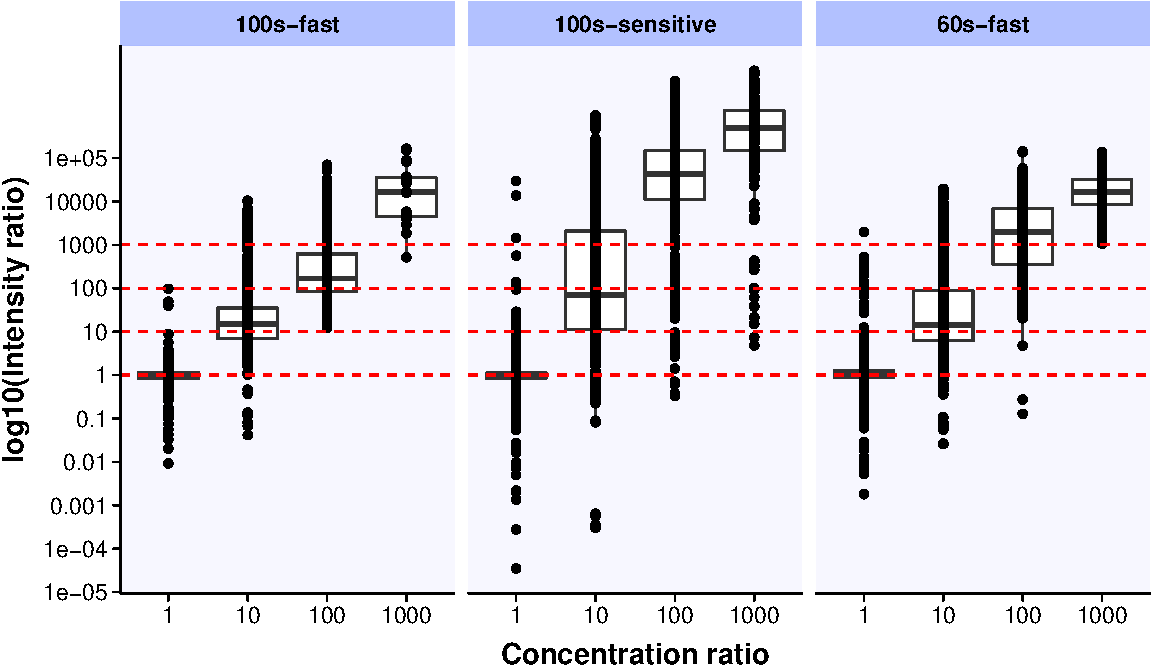
\includegraphics{BSA_files/figure-latex/unnamed-chunk-3-1.pdf}
\caption{\label{fig:unnamed-chunk-3}Intensity ratio between BSA peptides detected with each method. 100-s sensitive method has the least accurate intencity ratios.}
\end{figure}

\begin{figure}
\centering
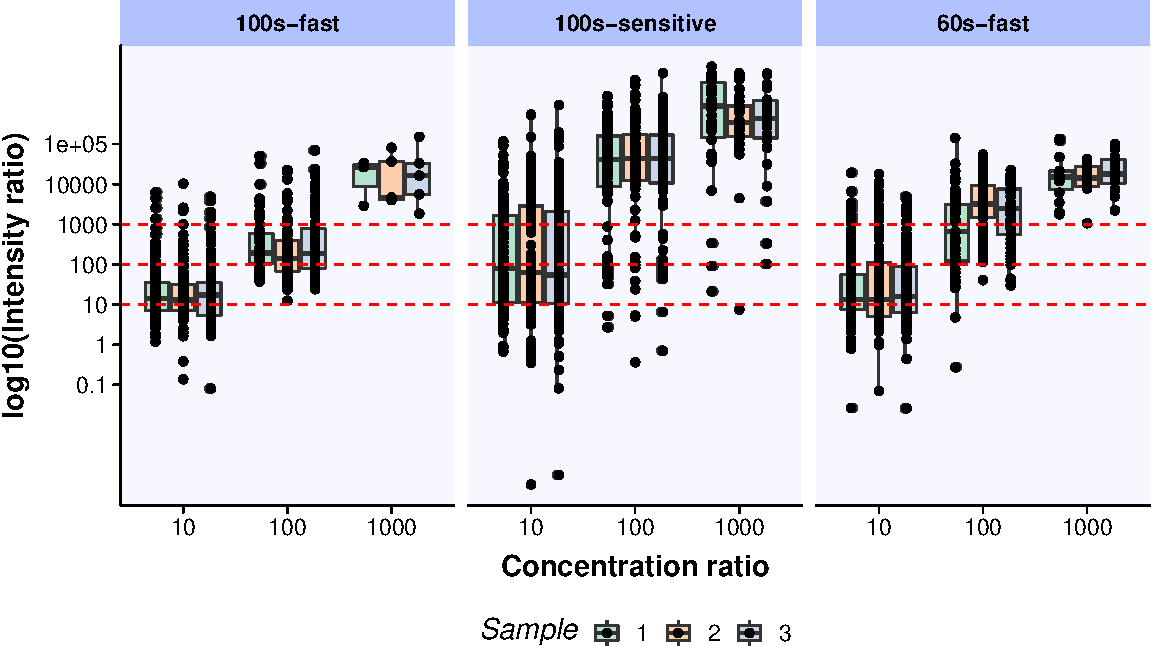
\includegraphics{BSA_files/figure-latex/unnamed-chunk-4-1.pdf}
\caption{\label{fig:unnamed-chunk-4}(Supplementary) Intensity ratio between BSA peptides detected with each method within one sample.}
\end{figure}

\hypertarget{bsa-hela}{%
\section{BSA + HeLa}\label{bsa-hela}}

\hypertarget{number-of-detected-peptides-1}{%
\subsection{Number of detected peptides}\label{number-of-detected-peptides-1}}

\begin{table}

\caption{\label{tab:tbl2}Number of BSA peptides detected in each sample.}
\centering
\begin{tabular}[t]{l|l|l|r}
\hline
run\_parameter & concentration & sample & n\_peptides\\
\hline
100s & 5000fmol & 1 & 115\\
\hline
100s & 5000fmol & 2 & 115\\
\hline
100s & 5000fmol & 3 & 114\\
\hline
100s & 500fmol & 1 & 99\\
\hline
100s & 500fmol & 2 & 99\\
\hline
100s & 500fmol & 3 & 103\\
\hline
100s & 50fmol & 1 & 65\\
\hline
100s & 50fmol & 2 & 65\\
\hline
100s & 50fmol & 3 & 70\\
\hline
100s & 5fmol & 1 & 58\\
\hline
100s & 5fmol & 2 & 46\\
\hline
100s & 5fmol & 3 & 53\\
\hline
60s & 5000fmol & 1 & 120\\
\hline
60s & 5000fmol & 2 & 121\\
\hline
60s & 5000fmol & 3 & 119\\
\hline
60s & 500fmol & 1 & 112\\
\hline
60s & 500fmol & 2 & 108\\
\hline
60s & 500fmol & 3 & 109\\
\hline
60s & 50fmol & 1 & 79\\
\hline
60s & 50fmol & 2 & 77\\
\hline
60s & 50fmol & 3 & 76\\
\hline
60s & 5fmol & 1 & 60\\
\hline
60s & 5fmol & 2 & 60\\
\hline
60s & 5fmol & 3 & 57\\
\hline
\end{tabular}
\end{table}

\newpage

\hypertarget{intensity-ratio-1}{%
\subsection{Intensity ratio}\label{intensity-ratio-1}}

\begin{figure}
\centering
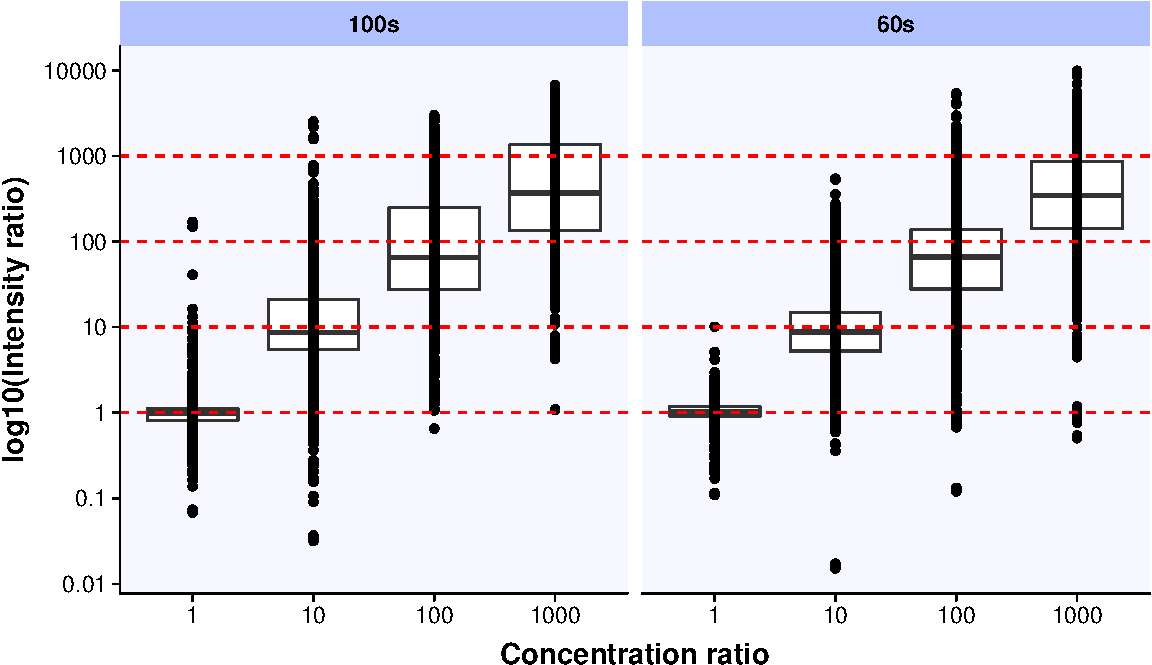
\includegraphics{BSA_files/figure-latex/unnamed-chunk-7-1.pdf}
\caption{\label{fig:unnamed-chunk-7}Intensity ratio between BSA peptides detected with each method. Intensity ratio in BSA+HeLa experiments are less biased than in BSA only experiments.}
\end{figure}

\begin{figure}
\centering
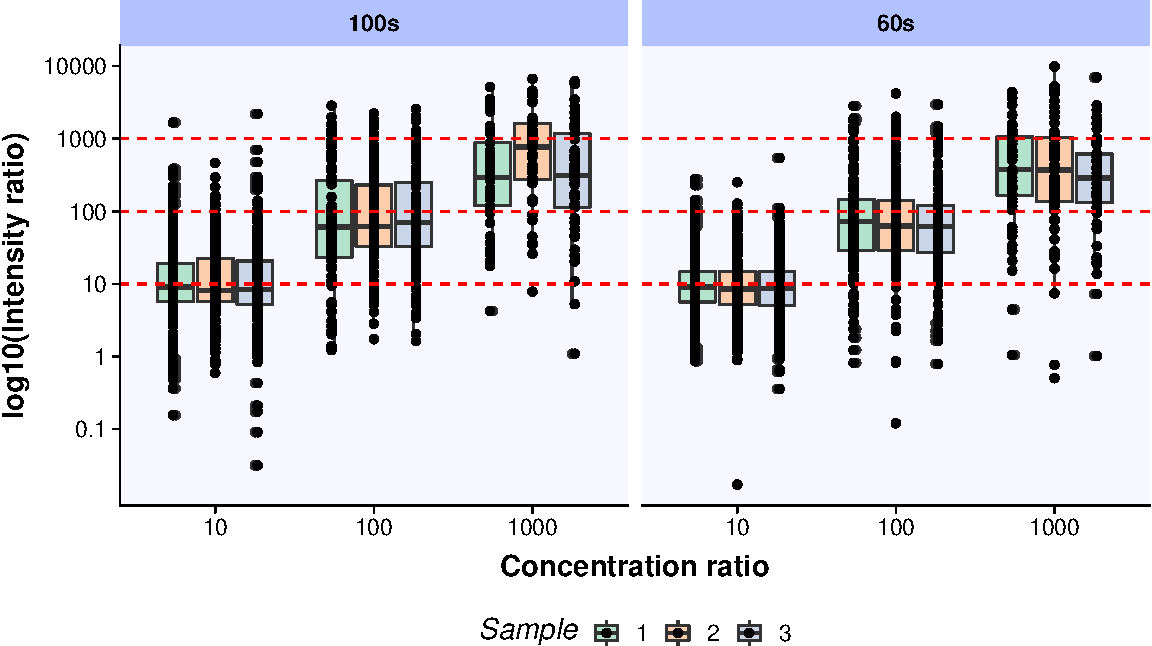
\includegraphics{BSA_files/figure-latex/unnamed-chunk-8-1.pdf}
\caption{\label{fig:unnamed-chunk-8}(Supplementary) Intensity ratio between BSA peptides detected with each method within one sample.}
\end{figure}

\end{document}
